\documentclass[xcolor=pdftex,dvipsnames,table]{presentation}
	\usetheme{Warsaw}
	\usecolortheme[RGB={100,0,0}]{structure}
%	\usefonttheme{structurebold}
%	\useoutertheme{smoothbars}
	\useinnertheme{rounded}

\usepackage{algpseudocode}
\usepackage[]{algorithmicx}
\usepackage{algorithm}

\def\ft{\mathcal{F}}
\algblockdefx[spawn]{Spawn}{EndSpawn}
[1]{\textbf{spawn process for} #1 \textbf{do}}
{\textbf{end spawn}}

\begin{document}

\title[Fast Fourier Transform]
{
	Fast Fourier Transform
}
%\subtitle{Text Here}
\author[McCarthy]
{
	Matt McCarthy
}
\institute[CNU]
{
	Christopher Newport University
}
\date[]
{
	CPSC 621\\
	November 30, 2015
}

\frame{\titlepage}

\begin{frame}
	\frametitle{Discrete Fourier Transform}

	\begin{definition}[Discrete Fourier Transform]
		Let $\mathbf{X}=\paren{x_0,x_1,\ldots,x_{n-1}}\in\CC^n$.
		Then the \textit{Discrete Fourier Transform of $\mathbf{X}$} is defined as $\mathbf{Y}=\paren{y_0,y_1,\ldots,y_{n-1}}$ where
		\[
			y_j:=\sum_{k=0}^{n-1}x_k \omega^{jk}
		\]
		with $\omega=e^{2\pi i/n}$.
		Furthermore, we denote $\mathbf{Y}=\ft(\mathbf{X})$.
	\end{definition}
	%\pause{}
	Complexity: $\Theta(n^2)$.
\end{frame}

\begin{frame}
	\frametitle{Slightly Faster Fourier Transform}
	If we assume $n$ is even, then by symbol pushing we get
	\begin{align*}
		y_j &=\sum_{k=0}^{n/2-1}x_{2k} \omega^{(2k)j} + \sum_{k=0}^{n/2-1}x_{2k+1}\omega^{(2k+1)j}\\
		&= \sum_{k=0}^{n/2-1}x_{2k} e^{2(2\pi i/n)jk} + \sum_{k=0}^{n/2-1}x_{2k+1}\omega^{j}e^{2(2\pi i/n)jk}\\
		&= \sum_{k=0}^{n/2-1}x_{2k} \paren{e^{2\pi i/n}}^{2jk} + \omega^{j}\sum_{k=0}^{n/2-1}x_{2k+1}\paren{e^{2\pi i/n}}^{2jk}
	\end{align*}
	%\pause{}
	Let $\tilde{\omega}=\omega^2$ and we have
	\[
		y_j = \sum_{k=0}^{n/2-1}x_{2k} {\tilde{\omega}}^{jk} + \omega^{j}\sum_{k=0}^{n/2-1}x_{2k+1}{\tilde{\omega}}^{jk}.
	\]
\end{frame}

\begin{frame}
	\frametitle{Fast Fourier Transform}

	If $n=2^k$ for some $k\in\ZZ^+$, then we can iterate this process using the following algorithm.

	%\pause
	The one-dimensional, unordered, radix 2, FFT algorithm.
	\begin{algorithmic}[1]
		\Function{R-FFT}{$\mathbf{X}$,$\mathbf{Y}$,$n$,$\omega$}
			\If{$n$=1}
				\State $y_0=x_0$
			\Else
				\State Let $\mathbf{Q}=\mathbf{0},\mathbf{T}=\mathbf{0}\in\CC^n$
				\State \Call{R-FFT}{$(x_0,x_2,\ldots,x_{n-2})$,$(q_0,q_2,\ldots,q_{n-2})$,$n/2$,$\omega^2$}
				\State \Call{R-FFT}{$(x_1,x_3,\ldots,x_{n-1})$,$(t_1,t_3,\ldots,t_{n-1})$,$n/2$,$\omega^2$}
				\ForAll{$j\in\set{0,1,\ldots,n-1}$}
					\State $y_j=q_{j\mod{n/2}}+\omega^i t_{j\mod{n/2}}$
				\EndFor
			\EndIf
		\EndFunction
	\end{algorithmic}
\end{frame}

\begin{frame}
	\frametitle{Fast Fourier Transform: Serial Analysis}

	\begin{itemize}
		\item Since $n=2^k$, we do $\lg n=k$ steps
		\item At the $m$th level of recursion we do $2^m$ FFTs of size $n/2^m$
		\begin{itemize}
			\item Each level is $\Theta(n)$
		\end{itemize}
		\item Thus, FFT is $\Theta(n\lg n)$.
	\end{itemize}
\end{frame}

\begin{frame}
	\frametitle{Iterative Formulation}
	\begin{algorithmic}[1]
		\Function{I-FFT}{$\mathbf{X}$,$\mathbf{Y}$,$n$}
			\State $t:=\lg n$
			\State $\mathbf{R}=\mathbf{X}$
			\For{$m=0$ to $t-1$}
				\State $\mathbf{S}=\mathbf{R}$
				\For{$l=0$ to $n-1$}
					\State Let $(b_0b_1\ldots b_{t-1})$ be the binary expansion of $l$
					\State $j:=(b_0\ldots b_{m-1}0b_{m+1}\ldots b_{t-1})$
					\State $k:=(b_0\ldots b_{m-1}1b_{m+1}\ldots b_{t-1})$
					\State $r_i:= s_j+s_k\omega^{(b_mb_{m-1}\ldots b_0 0\ldots0)}$
				\EndFor
			\EndFor
			\State $\mathbf{Y}:=\mathbf{R}$
		\EndFunction
	\end{algorithmic}
\end{frame}

\begin{frame}
	\frametitle{Binary-Exchange Algorithm: Pseudocode}

	\begin{algorithmic}[1]
		\Function{I-FFT}{$\mathbf{X}$,$\mathbf{Y}$,$n$}
			\State $t:=\lg n$
			\State $\mathbf{R}=\mathbf{X}$
			\Spawn{$l=0$ to $n-1$}
				\For{$m=0$ to $t-1$}
					\State Let $(b_0b_1\ldots b_{t-1})$ be the binary expansion of $l$
					\State $j:=(b_0\ldots b_{m-1}0b_{m+1}\ldots b_{t-1})$
					\State $k:=(b_0\ldots b_{m-1}1b_{m+1}\ldots b_{t-1})$
					\State $(s_j,s_k)\gets$\Call{Request}{$j$,$k$}
					\State $r_i:= s_j+s_k\omega^{(b_mb_{m-1}\ldots b_0 0\ldots0)}$
				\EndFor
			\EndSpawn
			\State \textbf{join all}
			\State $\mathbf{Y}:=\mathbf{R}$
		\EndFunction
	\end{algorithmic}
\end{frame}

\begin{frame}
	\frametitle{Binary-Exchange Algorithm: Assumptions}

	\begin{itemize}
		\item We need a bisection width of $\Theta(p)$ for $p$ processors.
		\item We have $p$ processors on a $\lg p$ dimensional hypercube.
		\begin{itemize}
			\item Analysis applicable to any network with $O(p)$ bandwidth.
		\end{itemize}
	\end{itemize}
\end{frame}

\begin{frame}
	\frametitle{Binary-Exchange Algorithm: One Task per Process}

	\begin{itemize}
		\item Output based decomposition
		\begin{itemize}
			\item Create $n$ tasks, task $l$ generates $y_l$
			\item Load $x_l$ into task $l$
			\item Map each task to a unique process ($n=p$)
		\end{itemize}
		\item Each process executes lines 7 to 10 of the iterative formulation
		\begin{itemize}
			\item Each process does this $\lg n$ times
		\end{itemize}
		\item To execute line 10, each process needs an element of $\mathbf{S}$ that differs from $l$ only by one bit.
		\item At iteration $m$, each process communicates with the process whose label differs from it at $m$th bit.
		\item Each iteration has one addition, multiplication, and exchange
		\item Ergo $T_p = \Theta(\lg n)$ and $C=pT_p=\Theta(n\lg n)$
	\end{itemize}
\end{frame}

\begin{frame}
	\frametitle{Binary-Exchange Algorithm: Multiple Tasks per Process}

	\begin{algorithmic}[1]
		\Function{I-FFT}{$\mathbf{X}$,$\mathbf{Y}$,$n$}
			\State $t:=\lg n$, $BLK:=n/p$
			\State $\mathbf{R}=\mathbf{X}$
			\Spawn{$l=0$ to $BLK-1$}
				\For{$c=l\cdot BLK$, to $l\cdot(BLK+1)$}
					\For{$m=0$ to $t-1$}
						\State Let $(b_0b_1\ldots b_{t-1})$ be the binary expansion of $c$
						\State $j:=(b_0\ldots b_{m-1}0b_{m+1}\ldots b_{t-1})$
						\State $k:=(b_0\ldots b_{m-1}1b_{m+1}\ldots b_{t-1})$
						\State $(s_j,s_k)\gets$\Call{Request}{$j$,$k$}
						\State $r_i:= s_j+s_k\omega^{(b_mb_{m-1}\ldots b_0 0\ldots0)}$
					\EndFor
				\EndFor
			\EndSpawn
			\State \textbf{join all}
			\State $\mathbf{Y}:=\mathbf{R}$
		\EndFunction
	\end{algorithmic}
\end{frame}

\begin{frame}
	\frametitle{Binary-Exchange Algorithm: Example}

	\begin{figure}
		\centering
		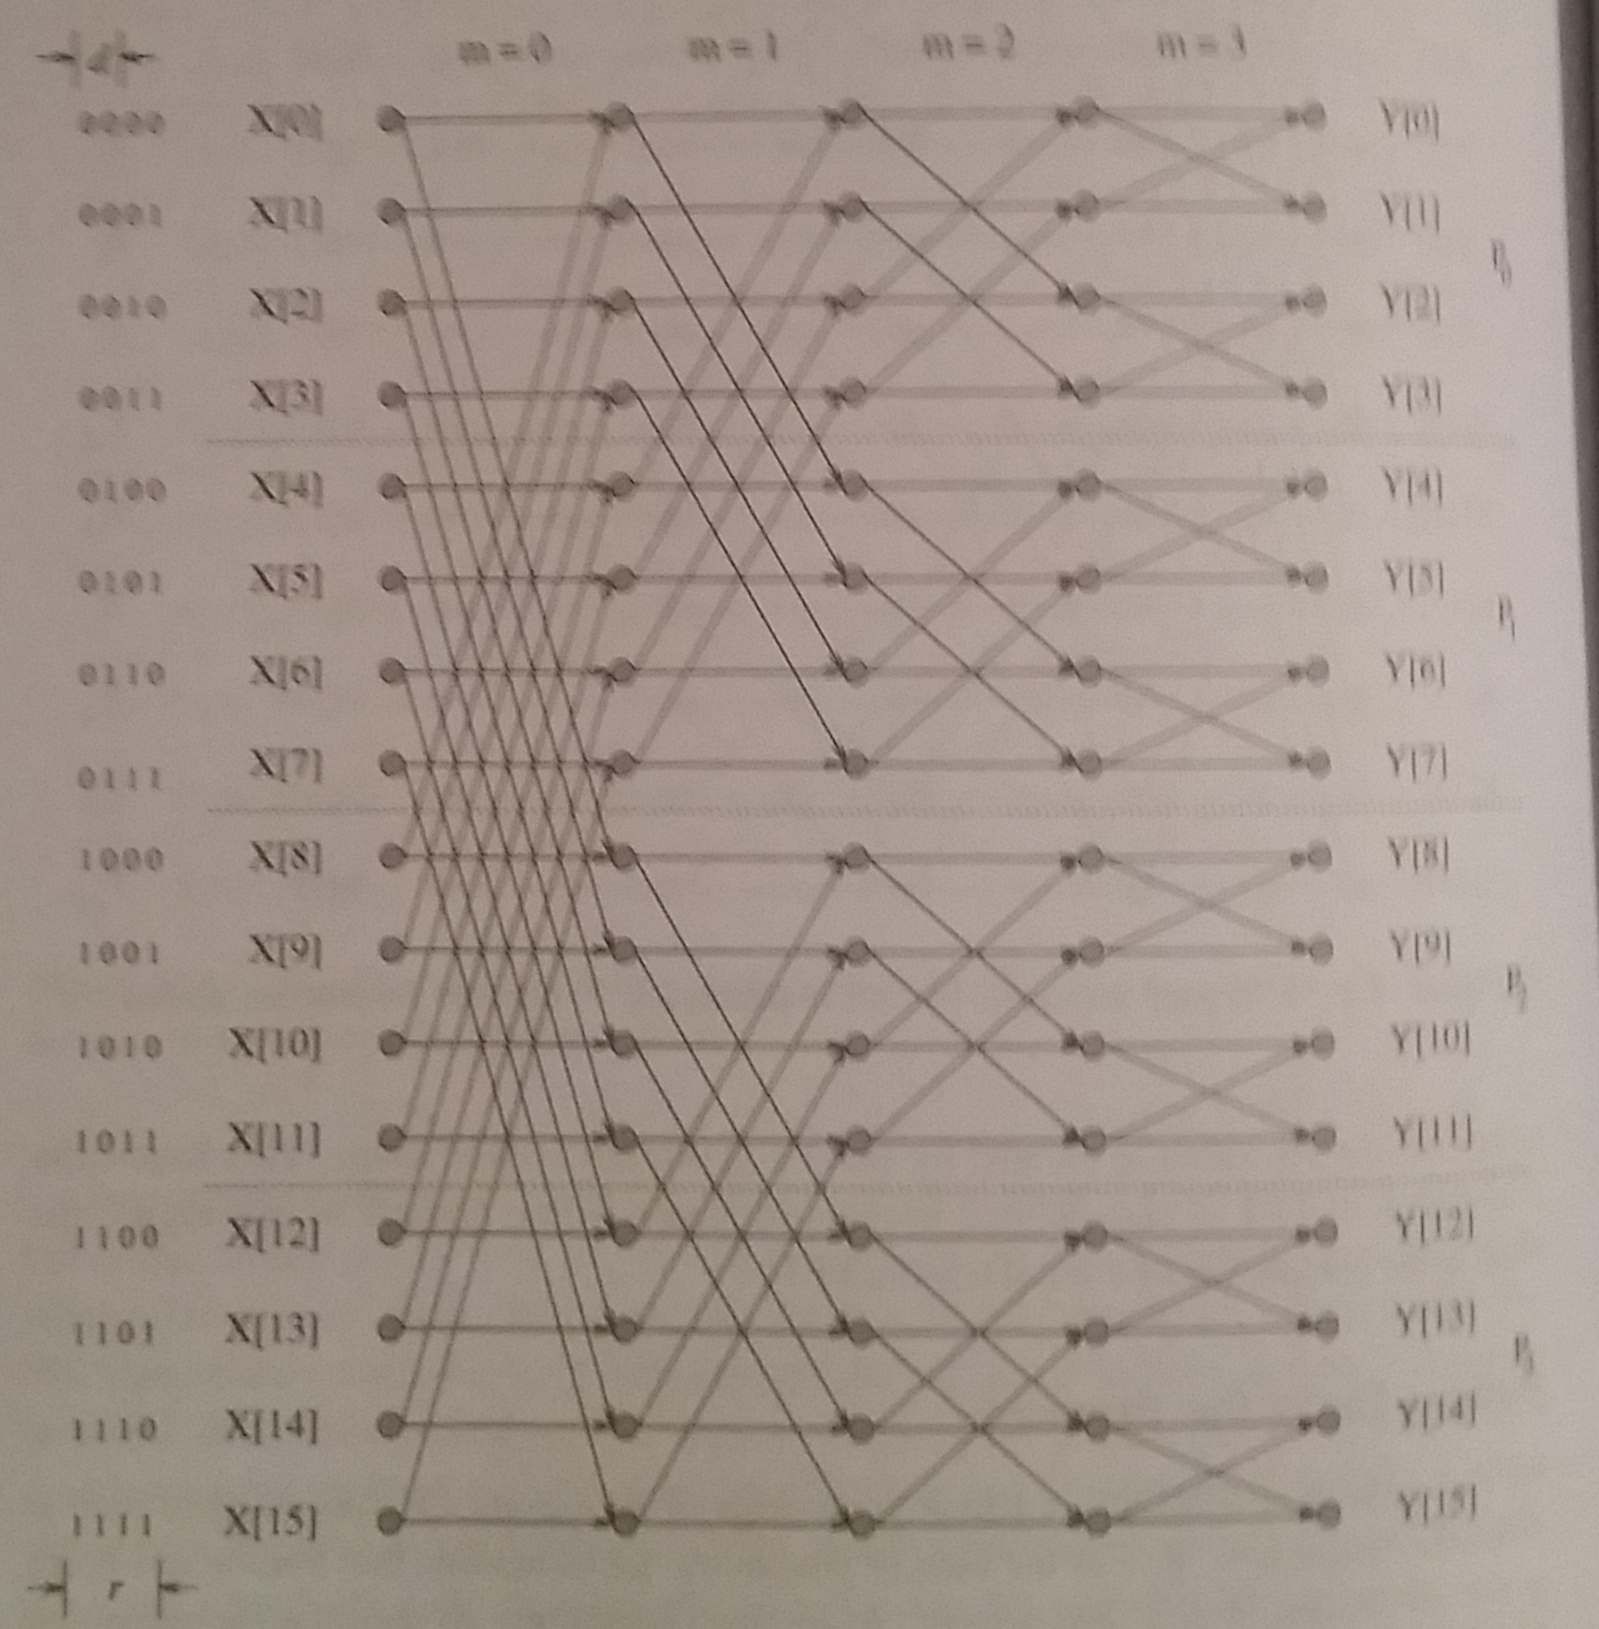
\includegraphics[scale=0.1]{fft.jpg}
		\caption{An example of FFT with $n=16$ and $p=4$}
	\end{figure}
\end{frame}

\begin{frame}
	\frametitle{Binary-Exchange Algorithm: Analysis 2}

	\begin{itemize}
		\item Assume both $n=2^t$ and $p=2^d$
		\item Same procedure as previous analysis
		\item However, interprocessor communication happpens on first $d$ steps, and not at all on the remaining steps
		\item Communication cost:
		\[
			t_s\lg p+ t_w\frac{n}{p}\lg p
		\]
		\item Computation cost:
		\[
			t_c\frac{n}{p}\lg n
		\]
	\end{itemize}
\end{frame}

\begin{frame}
	\frametitle{Binary-Exchange Algorithm: Analysis 2}

	\begin{itemize}
		\item Total runtime:
		\[
			T_p = t_c\frac{n}{p}\lg n + t_s\lg p+ t_w\frac{n}{p}\lg p
		\]
		\item Cost:
		\[
			C=pT_p=t_c n\lg n +t_s \lg p +t_w n\lg p
		\]
		\item Cost optimal for all $p\leq n$ ($C=O(n\lg n)$)
		\item Speedup:
		\[
			S=\frac{pn\lg n}{n\lg n+(t_s/t_c)p\lg p+(t_w/t_c)n\lg p}
		\]
		\item Efficiency:
		\[
			E=\paren{1+\frac{t_sp\lg p}{t_c n\lg n}+\frac{t_w\lg p}{t_c\lg n}}^{-1}
		\]
	\end{itemize}
\end{frame}

\begin{frame}
	\frametitle{Binary-Exchange Algorithm: Mesh Analysis}

	\begin{itemize}
		\item Computation cost remains the same.
		\[
			t_c\frac{n}{p}\lg n
		\]
		\item Row/Column Communication cost:
		\[
			\sum_{m=0}^{d/2-1} t_s+t_w\frac{n}{p}2^m
		\]
		\item Total runtime:
		\[
			T_p \approx t_c\frac{n}{p}\lg n+ t_s\lg p +2t_w\frac{n}{\sqrt{p}}
		\]
	\end{itemize}
\end{frame}

\begin{frame}
	\frametitle{Binary-Exchange Algorithm: Mesh Analysis}

	\begin{itemize}
		\item Speedup
		\[
			S\approx \frac{pn\lg n}{n\lg n+(t_s/t_c)p\lg p + 2(t_w/t_c)n\sqrt{p}}
		\]
		\item Efficiency
		\[
			E\approx \paren{1+\frac{t_s p\lg p}{t_c n\lg n}+\frac{2t_w\sqrt{p}}{t_c\lg n}}^{-1}
		\]
		\item Cost
		\[
			C=pT_p\approx t_c n\lg n+ t_s p\lg p +2t_w n\sqrt{p}
		\]
		\item Cost optimal iff $\sqrt{p}=O(\lg n)$.
	\end{itemize}
\end{frame}

\begin{frame}
	\frametitle{Binary-Exchange Algorithm: Duplicated Work}

	\begin{algorithmic}[1]
		\Function{I-FFT}{$\mathbf{X}$,$\mathbf{Y}$,$n$}
			\State $t:=\lg n$, $BLK:=n/p$
			\State $\mathbf{R}=\mathbf{X}$
			\Spawn{$l=0$ to $BLK-1$}
				\For{$c=l\cdot BLK$, to $l\cdot(BLK+1)$}
					\For{$m=0$ to $t-1$}
						\State Let $(b_0b_1\ldots b_{t-1})$ be the binary expansion of $c$
						\State $j:=(b_0\ldots b_{m-1}0b_{m+1}\ldots b_{t-1})$
						\State $k:=(b_0\ldots b_{m-1}1b_{m+1}\ldots b_{t-1})$
						\State $(s_j,s_k)\gets$\Call{Request}{$j$,$k$}
						\State $r_i:= s_j+s_k\omega^{(b_mb_{m-1}\ldots b_0 0\ldots0)}$
					\EndFor
				\EndFor
			\EndSpawn
			\State \textbf{join all}
			\State $\mathbf{Y}:=\mathbf{R}$
		\EndFunction
	\end{algorithmic}
\end{frame}

\begin{frame}
	\frametitle{Extra Notes}

	\begin{itemize}
		\item Two dimensional transpose algorithm
		\begin{itemize}
			\item Uses matrix transposition to do FFT
			\item Total exchange
			\item Works for low-bandwidth situations
			\item Cost optimal iff $n\lg n = \Omega(p^2\lg p)$
			\item Preffered over binary-exchange if $t_s$ is small
		\end{itemize}
	\end{itemize}
\end{frame}

\begin{frame}[allowframebreaks]
\frametitle{References}
	\begin{thebibliography}{10}
		\bibitem{par-book}
		Grama et. al.
		\newblock{} Introduction to Parallel Computing.
		\newblock{} Pearson Education.
	\end{thebibliography}
\end{frame}

\end{document}
